\hypertarget{python-ux7b80ux4ecb}{%
\subsection{Python 简介}\label{python-ux7b80ux4ecb}}

Python 是著名的 ``龟叔''Guido van Rossum 在 1989
年圣诞节期间,为了打发无聊的圣诞节而编写的一个编程语言。

现在,全世界差不多有 600 多种编程语言,但流行的编程语言也就那么 20
来种。如果你听说过 TIOBE
排行榜,你就能知道编程语言的大致流行程度。这是最近 10 年最常用的 10
种编程语言的变化图:

 
 \begin{figure}[htp]
	\centering
	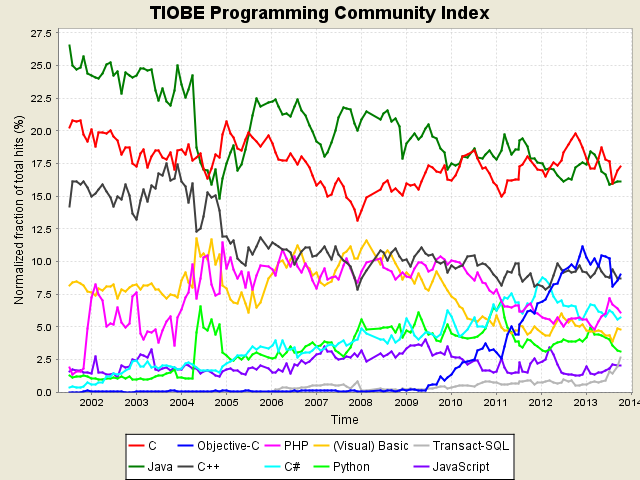
\includegraphics[width=0.6\linewidth]{fig/9212153960043840.png}
\end{figure}


总的来说,这几种编程语言各有千秋。C
语言是可以用来编写操作系统的贴近硬件的语言,所以,C
语言适合开发那些追求运行速度、充分发挥硬件性能的程序。而 Python
是用来编写应用程序的高级编程语言。

当你用一种语言开始作真正的软件开发时,你除了编写代码外,还需要很多基本的已经写好的现成的东西,来帮助你加快开发进度。比如说,要编写一个电子邮件客户端,如果先从最底层开始编写网络协议相关的代码,那估计一年半载也开发不出来。高级编程语言通常都会提供一个比较完善的基础代码库,让你能直接调用,比如,针对电子邮件协议的
SMTP 库,针对桌面环境的 GUI
库,在这些已有的代码库的基础上开发,一个电子邮件客户端几天就能开发出来。

Python
就为我们提供了非常完善的基础代码库,覆盖了网络、文件、GUI、数据库、文本等大量内容,被形象地称作
``内置电池(batteries included)''。用 Python
开发,许多功能不必从零编写,直接使用现成的即可。

除了内置的库外,Python
还有大量的第三方库,也就是别人开发的,供你直接使用的东西。当然,如果你开发的代码通过很好的封装,也可以作为第三方库给别人使用。

许多大型网站就是用 Python 开发的,例如
YouTube、\href{http://instagram.com/}{Instagram},还有国内的\href{http://www.douban.com/}{豆瓣}。很多大公司,包括
Google、Yahoo 等,甚至
\href{http://www.nasa.gov/}{NASA}(美国航空航天局)都大量地使用 Python。

龟叔给 Python 的定位是 ``优雅''、``明确''、``简单'',所以 Python
程序看上去总是简单易懂,初学者学
Python,不但入门容易,而且将来深入下去,可以编写那些非常非常复杂的程序。

总的来说,Python
的哲学就是简单优雅,尽量写容易看明白的代码,尽量写少的代码。如果一个资深程序员向你炫耀他写的晦涩难懂、动不动就几万行的代码,你可以尽情地嘲笑他。

那 Python 适合开发哪些类型的应用呢?

首选是网络应用,包括网站、后台服务等等;

其次是许多日常需要的小工具,包括系统管理员需要的脚本任务等等;

另外就是把其他语言开发的程序再包装起来,方便使用。

最后说说 Python 的缺点。

任何编程语言都有缺点,Python 也不例外。优点说过了,那 Python
有哪些缺点呢?

第一个缺点就是运行速度慢,和 C 程序相比非常慢,因为 Python
是解释型语言,你的代码在执行时会一行一行地翻译成 CPU
能理解的机器码,这个翻译过程非常耗时,所以很慢。而 C
程序是运行前直接编译成 CPU 能执行的机器码,所以非常快。

但是大量的应用程序不需要这么快的运行速度,因为用户根本感觉不出来。例如开发一个下载
MP3 的网络应用程序,C 程序的运行时间需要 0.001 秒,而 Python
程序的运行时间需要 0.1 秒,慢了 100 倍,但由于网络更慢,需要等待 1
秒,你想,用户能感觉到 1.001 秒和 1.1 秒的区别吗?这就好比 F1
赛车和普通的出租车在北京三环路上行驶的道理一样,虽然 F1 赛车理论时速高达
400 公里,但由于三环路堵车的时速只有 20
公里,因此,作为乘客,你感觉的时速永远是 20 公里。

 
 \begin{figure}[htp]
	\centering
	
\includegraphics[width=0.6\linewidth]{fig/9230247568328960.png}
\end{figure}


第二个缺点就是代码不能加密。如果要发布你的 Python
程序,实际上就是发布源代码,这一点跟 C 语言不同,C
语言不用发布源代码,只需要把编译后的机器码(也就是你在 Windows 上常见的
xxx.exe 文件)发布出去。要从机器码反推出 C
代码是不可能的,所以,凡是编译型的语言,都没有这个问题,而解释型的语言,则必须把源码发布出去。

这个缺点仅限于你要编写的软件需要卖给别人挣钱的时候。好消息是目前的互联网时代,靠卖软件授权的商业模式越来越少了,靠网站和移动应用卖服务的模式越来越多了,后一种模式不需要把源码给别人。

再说了,现在如火如荼的开源运动和互联网自由开放的精神是一致的,互联网上有无数非常优秀的像
Linux 一样的开源代码,我们千万不要高估自己写的代码真的有非常大的
``商业价值''。那些大公司的代码不愿意开放的更重要的原因是代码写得太烂了,一旦开源,就没人敢用他们的产品了。

 
 \begin{figure}[htp]
	\centering
	
\includegraphics[width=0.6\linewidth]{fig/9230254446989120.png}
\end{figure}


当然,Python 还有其他若干小缺点,请自行忽略,就不一一列举了。

